\documentclass[10pt]{report}

\usepackage{subcaption} % for subfigures
\usepackage{amsthm} % for QED
\usepackage{mathtools} % for delimiter

\usepackage{listings} % for code
\lstset{ 
	language=R,
	basicstyle=\ttfamily,
	numbers=none,
	stepnumber=1,
	numbersep=8pt,
	showspaces=false,
	showstringspaces=false,
	showtabs=false,
	frame=single,
	tabsize=2,
	captionpos=t,
	breaklines=true,
	breakatwhitespace=false
} 

\usepackage{float} % for figure [H]
\usepackage{booktabs} % for tabular
\usepackage{caption} % for \caption*
\usepackage[export]{adjustbox} % for valign=t
\usepackage{array} % for column type m
\usepackage{verbatim}
\usepackage{graphicx}
%\graphicspath{ {imgs/} }
\usepackage{fancyhdr}
\usepackage{amssymb}
\usepackage{amsmath}

%%%%%% Pagination
\setlength{\topmargin}{-.3 in}
\setlength{\oddsidemargin}{0in}
\setlength{\evensidemargin}{0in}
\setlength{\textheight}{9.in}
\setlength{\textwidth}{6.5in}

%Title page
\newcommand{\hwTitle}{Homework \#2}
\newcommand{\hwCourse}{Applied Statistics/Regression}
\newcommand{\hmwkClassInstructor}{Professor Lulu Kang}

\title{
	\vspace{2in}
	\textmd{\textbf{\hwCourse\\\hwTitle}}\\
	\vspace{0.3in}\large{\textit{\hmwkClassInstructor}}
	\vspace{3in}
}

%\title{Homework 1}
\author{\textbf{Zhihao Ai}}
\date{}

%Header setting. 
\pagestyle{fancy}
\fancyhead[L]{Zhihao Ai}
\fancyhead[C]{Math 484}
\fancyhead[R]{Homework 2}
%%%%%%

%Global setting.
%\everymath{\displaystyle}
\setlength\parindent{0pt}

%Custom general commands.
\newcommand{\ds}{\displaystyle}
\newcommand{\ts}{\textstyle}
\newcommand{\f}[1] {f\left(#1\right)}
\newcommand{\eva}[2] {\left. #1 \right|_{#2}}
\newcommand{\dintt}[4] {\int_{#1}^{#2} #3 d#4}

\newcolumntype{N}{ >$ c <$}
\newcolumntype{M}[1]{>{\centering\arraybackslash $}m{#1}<{$}}

\newcommand{\abs}[1] {\left| #1 \right|}

\DeclarePairedDelimiter\autoparen{(}{)}
\newcommand{\pa}[1]{\autoparen*{#1}}
\DeclarePairedDelimiter\autodvert{\Vert}{\Vert}
\DeclarePairedDelimiter{\floor}{\lfloor}{\rfloor}
\newcommand{\norm}[1]{\autodvert*{#1}}

\newcommand{\var}{\text{var}}

\begin{document}

\maketitle

\subsection*{Ex 2.27}
Refer to Muscle mass Problem 1.27.
\begin{enumerate}
	\item [a.]
	Conduct a test to decide whether or not there is negative linear association between amount of muscle mass and age. Control the risk of Type I error at .05. State the alternatives, decision rule, and conclusion. What is the \textit{P}-value of the test?
	
	The two alternatives are:
	\begin{align*}
		H_0: \beta_1 \ge 0\\
		H_a: \beta_1 < 0
	\end{align*}
	The test statistic is $t^* = \frac{\hat{\beta}_1}{s\{\hat{\beta}_1\}}$ and the decision rule is
	\begin{align*}
		\text{If } t^* \ge -t_{\alpha, n-2} = -1.67, \text{ conclude } H_0\\
		\text{If } t^* < -t_{\alpha, n-2} = -1.67, \text{ conclude } H_a
	\end{align*}
	\lstinputlisting{27a.txt}
	Since $t^* = -13.19 < -1.67$, we conclude $H_a$, that there is a negative linear association between the two attributes. The \textit{P}-value of the test is $0+$.
	
	\item [b.]
	The two-sided \textit{P}-value for the test whether $\beta_0 = 0$ is $0+$. Can it now be concluded that $b_0$ provides relevant information on the amount of muscle mass at birth for a female child?
	
	Since the data is sampled from women aged from 40 to 79, the amount of muscle mass for female children at birth is not included. Also it is not reasonable to infer the muscle mass of children from that of adults. Therefore, it cannot be concluded that $b_0$ provides relevant information.
	
	\item [c.]
	Estimate with a 95 percent confidence interval the difference in expected muscle mass for women whose ages differ by one year. Why is it not necessary to know the specific ages to make this estimate?
	\[
	s\{\hat{\beta}_1\} = \frac{\sigma^2}{S_{xx}} = \frac{\hat{\sigma}^2}{S_{xx}} = \frac{SSE/(n-2)}{S_{xx}} = 0.0902
	\]
	 Also we have $t_{0.025, 58} = 2.0017$. So the 95 percent confidence interval is $(\hat{\beta}_1 - t_{0.025, 58}\cdot s\{\hat{\beta}_1\}, \hat{\beta}_1 + t_{0.025, 58}\cdot s\{\hat{\beta}_1\}) = (-1.37, -1.01)$. Since the confidence interval is calculated based on the distribution of $\hat{\beta}_1$ and the $t$ multiple, the specific $x$ value is not needed.
\end{enumerate}

\subsection*{Ex 1.19}
\textbf{Grade point average.} The director of admissions of a small college selected 120 students at random from the new freshman class in a study to determine whether a student's grade point average(GPA) at the end of the freshman year(Y) can be predicted from the ACT test score(X). The results of the study follow. Assume that first-order regression model(1.1) is appropriate.
\begin{enumerate}
	\item [a.]
	Obtain the least squares estimates of $\beta_0$ and $\beta_1$, and state the estimated regression function.
	\lstinputlisting{19a.txt}
	The least square estimates of $\beta_0$ and $\beta_1$ are $\hat{\beta}_0 = 2.11, \hat{\beta}_1 = 0.04$. The estimated regression function is $\hat{Y} = 0.04x + 2.11$.
	
	\item [b.]
	Plot the estimated regression function and the data. Does the estimated regression function appear to fit the data well?
	\begin{figure}[H]
		\centering
		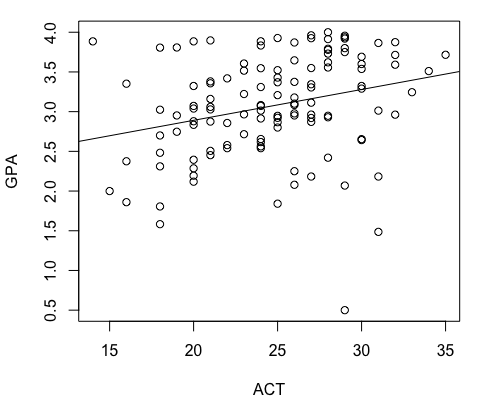
\includegraphics[width=.6\linewidth]{19b.png}
	\end{figure}
	This function generally gives not a very good but acceptable fit.
	
	\item [c.]
	Obtain a point estimate of the mean freshman GPA for students with ACT test score $X=30$.
	
	A point estimate is $\hat{Y}(30) = 0.04(30) + 2.11 = 3.31$.
	
	\item [d.]
	What is the point estimate of the change in the mean response when the entrance test score increses by one point?
	
	The point estimate is $\hat{\beta}_1 = 2.11$.
\end{enumerate}

\subsection*{Ex 2.13}
Refer to Grade point average Problem 1.19.
\begin{enumerate}
	\item [a.]
	Obtain a 95 percent interval estimate of the mean freshman GPA for students whose ACT test score is 28. Interpret your confidence interval.
	\lstinputlisting{13a.txt}
	The interval is $(3.06,3.34)$, meaning there is 95 precent probability that the mean GPA for students whose ACT test score is 28 would fall into this interval.
	
	\item [b.]
	Mary Jones obtained a score of 28 on the entrance test. Predict her freshman GPA using a 95 percent prediction interval. Interpret your prediction interval.
	\lstinputlisting{13b.txt}
	The interval is $(1.96,4.44)$, meaning there is 95 precent probability that her freshman GPA would fall into this interval.
	
	\item [c.]
	Is the prediction interval in part (b) wider than the confidence interval in part (a)? Should it be?
	
	Yes, it is wider than that in part (a). It should be because the interval in part (a) is to  predict the mean response for $X=28$ while the interval in part (b) is to predict $y$ for $X=28$ and takes into account the variation of error.
	
	\item [d.]
	Determine the boundary values of the 95 percent confidence band for the regression line when $X_h = 28$. Is your confidence band wider at this point than the confidence interval in part (a)? Should it be?
	\[
	s\{\hat{Y}\} = \sqrt{\hat{\sigma}^2 \pa{\frac{1}{n} - \frac{(x_h-\bar{x})^2}{S_{xx}}}} = \sqrt{\frac{RSS}{n-2}\pa{\frac{1}{n} - \frac{(x_h-\bar{x})^2}{S_{xx}}}} = 0.0706
	\]
	Since $W = \sqrt{2F_{0.95, 2, 118}} = 2.479$, the boundary values of the confidence band for $X_h = 28$ are $\hat{Y} \pm W\cdot s\{\hat{Y}\}$. Hence, the interval is $(3.026, 3.376)$. It is wider that that in part (b) and it should be because the confidence band must encompass the entire regression line, whereas the confidence limits for $E(\hat{Y})$ at $X = 28$ apply only at the single level of $X = 28$.
\end{enumerate}

\subsection*{Ex 2.23}
Refer to Grade point average Problem 1.19.
\begin{enumerate}
	\item [a.]
	Set up the ANOVA table.
	\lstinputlisting{23a.txt}
	
	\item [b.]
	What is estimated by $MSR$ in your ANOVA table? by $MSE$? Under what condition do $MSR$ and $MSE$ estimate the same quantity?
	
	The mean square for act which is 3.5878 is estimated by $MSR$. The mean square for residuals which is 0.3883 is estimated by $MSE$. When $\beta_1 = 0$, $MSR$ and $MSE$ will estimate the same quantity.
	
	\item [c.]
	Conduct an $F$ test of whether or not $\beta_1 = 0$. Control the $\alpha$ risk at .01. State the alternatives, decision rule, and conclusion.
	
	The two alternatives are:
	\begin{align*}
		H_0: \beta_1 = 0\\
		H_a: \beta_1 \ne 0
	\end{align*}
	The test statistic is
	\[
	F^* = \frac{SSR/\sigma^2}{1} \div \frac{SSE/\sigma^2}{n-2} = \frac{MSR}{MSE}
	\]
	The decision rule is
	\begin{align*}
		\text{If } F^* \le F_{\alpha, 1, n-2} = 6.85, \text{ conclude } H_0\\
		\text{If } F^* > F_{\alpha, 1, n-2} = 6.85, \text{ conclude } H_a
	\end{align*}
	Given by the ANOVA table, $MSR = 3.59$ and $MSE = 0.39$. Since $F^* = 3.5878/0.3883 = 9.24 > 6.85$, we conclude $H_a$, that $\beta_1 \ne 0$.
	
	\item [d.]
	What is the absolute magnitude of the reduction in the variation of $Y$ when $X$ is introduced into the regression model? What is the relative reduction? What is the name of the latter measure?
	
	\lstinputlisting{23d.txt}
	The absolute magnitude of the reduction is $SSR = 3.588$. The relative reduction is $\frac{SSR}{SSTO} = \frac{3.588}{3.588+45.818} = 0.07262$. The latter measure is $R^2$.
	
	\item [e.]
	Obtain $r$ and attach the appropriate sign.
	
	$r = +\sqrt{R^2} = 0.269$ since the sign of $\hat{\beta}_1$ is positive.
	
	\item [f.]
	Which measure, $R^2$ or $r$, has the more clear-cut operational interpretation? Explain.
	
	$R^2$, because it shows the proportionate reduction of total variation associated with the use of the predictor variable $X$.
\end{enumerate}

{\large\bf Show that for simple linear regression, the t-ratio, $t=\frac{\hat{\beta}_1}{s.e.(\hat{\beta}_1)}$ and the F-ratio, $F=\frac{SS_{reg}}{\hat{\sigma}^2}$ has the relationship, $t^2=F$.}
\begin{align*}
	SS_{reg}
	&= \sum_{i=1}^{n} (\hat{y}_i - \bar{y})^2 
	= \sum_{i=1}^{n} (\hat{\beta}_1 x_i + \hat{\beta}_0 - \bar{y})^2 
	= \sum_{i=1}^{n} (\hat{\beta}_1 x_i + \bar{y} - \hat{\beta}_1 \bar{x} - \bar{y})^2\\
	&= \sum_{i=1}^{n} (\hat{\beta}_1 (x_i - \bar{x}))^2
	= \hat{\beta}_1^2 \sum_{i=1}^{n} (x_i - \bar{x})^2\\
	F
	&= \frac{SS_{reg}}{\hat{\sigma}^2}
	= \frac{\hat{\beta}_1^2 \sum_{i=1}^{n} (x_i - \bar{x})^2}{\hat{\sigma}^2}
	= \frac{\hat{\beta}_1^2}{\hat{\sigma}^2/S_{xx}}
	= \pa{\frac{\hat{\beta}_1}{s/\sqrt{S_{xx}}}}^2
	= \pa{\frac{\hat{\beta}_1}{s.e.(\hat{\beta}_1)}}^2
	= t^2
\end{align*}
\qed

\end{document}
